This section describes the data storage layer of this project, namely \gls{HopsFS}. \gls{HopsFS} is Hopsworks's evolution of \gls{HDFS}, a distributed file system. \gls{HopsFS} complexity will be broken down into parts, providing not only a great understanding of the tool but also a comparison with common alternatives, namely cloud object stores.

\subsection{File storage vs. Object storage vs. Block storage}
\label{subsec:file_vs_obj_vs_block}

Data can be stored and organized in physical storages, such as \glspl{HDD} and/or \glspl{SSD}, in three major ways: (1)~Files, (2)~Objects, and (3)~Blocks. For each one, the technique is briefly described and then a comparative table is shown (Table \ref{tab:storagecomparison}). This subsection is a rework according to the author's understanding of three articles coming from major cloud providers (Amazon, Google, and IBM) \cite{BlockVsFile, HowObjectVs, ObjectVsFile2021}.

\subsubsection*{File storage}

File storage is a hierarchical data storage technique that stores data into files. A file is a collection of data characterized by a file extension (e.g. ".txt", ".png", ".csv", ".parquet") that indicates how the data contained is organized. Every file is contained within a directory, that can contain other files or other directories (called "subdirectories"). In many file storage systems directories are called "folders". 

This type of structure, very common in modern \glspl{PC}, simplifies locating and retrieving a single file and its flexibility allows it to store any type of data. However, its hierarchical structure requires that to access a file, its exact location should be known. This restriction decreases the scaling possibilities of the system, where a large amount of data needs to be retrieved at the same time.

Overall, this solution is still vastly popular in user-facing storage applications (e.g. Dropbox, Google Drive, One Drive) and \glspl{PC} thanks to its intuitive structure and ease of use. On the other hand, other options are preferred for managing large quantities of data, due to its lack in scalability. \\[3mm]
\noindent\textbf{Advantages}
\begin{itemize}
    \item Ideal for small-scale operations (low latency, efficient folderization).
    \item User familiarity and ease of management.
    \item File-level access permissions and locking capabilities.
\end{itemize}

\noindent\textbf{Disadvantages}
\begin{itemize}
    \item Difficult to scale due to deep folderization.
    \item Inefficient in storing unstructured data.
    \item Limitations in scalability due to reaching device or network capacity.
\end{itemize}

\subsubsection*{Object storage}

Object storage is a flat data storage technique that stores data into objects. An object is an isolated container associated with metadata, i.e. a set of attributes that describe the data e.g. a unique identifier, object name, size, and creation date. Metadata is used to retrieve the data more easily, allowing for queries that retrieve large quantities of data simultaneously, e.g. all data that was created on a specific date. 

The flat structure of Object storage, where all objects are in the same container called a bucket, is ideal for managing large quantities of unstructured data (e.g. videos, images). This structure is also easier to scale as it can be replicated easily across multiple regions allowing faster access in different areas of the world, and fault tolerance to hardware failure.

On the other hand, objects cannot be altered once created, and in case of a change must recreated. Also, object stores are not ideal for transactional operations as objects cannot have a locking mechanism. Lastly, object stores have slower writing performance compared to file or block storage solutions.

Overall, this solution is widely when high scalability is required (e.g. social networks, and video streaming apps) thanks to its flat structure and use of metadata. On the other hand, other options are preferred when transactional operations are required, or high performance on a small number of files that change frequently is necessary. \\[3mm]
\noindent\textbf{Advantages}
\begin{itemize}
    \item Potential unlimited scalability.
    \item Effective use of metadata enabling advanced queries.
    \item Cost-efficient storage for all types of data (also unstructured).
\end{itemize}

\noindent\textbf{Disadvantages}
\begin{itemize}
    \item Absence of file locking mechanisms.
    \item Low performance (increased latency and processing overhead).
    \item Lacks data update capabilities (only recreation).
\end{itemize}

\subsubsection*{Block storage}

Block storage is a data storage technique that divides data into blocks of fixed size that can be read or written individually. Each block is associated with a unique identifier and it is then stored on a physical server (note that a block can be stored in different \glspl{OS}). When the user requests the data saved, the block storage retrieves the data from the associated blocks and then re-assembles the data of the blocks into a single unit. The block storage also manages the physical location of the block, saving a block where is more efficient.

Block storage is very effective for systems needing fast access and low latency. This architecture is compatible with frequent changes, unlike object storage.

On the other hand, block storage achieves its speed by operating at a low level on physical systems, so the cost of the architecture is strictly bound to the storage and servers used, not allowing the architecture to scale according to its demands. \\[3mm]
\noindent\textbf{Advantages}
\begin{itemize}
    \item High performance (low latency).
    \item Reliable self-contained storage units.
    \item Data stored can be modified easily.
\end{itemize}

\noindent\textbf{Disadvantages}
\begin{itemize}
    \item Lack of metadata brings limitations in data searchability.
    \item High cost to scale the infrastructure.
\end{itemize}

\begin{table}[!ht]
    \begin{center}
      \caption[Data storage features comparison]{Data storage features comparison. Table inspired by major cloud providers articles \cite{BlockVsFile,HowObjectVs}.}
      \label{tab:storagecomparison}
      \begin{tabular}{cccc} % <-- Alignments: 1st column left, 2nd middle, with vertical lines in between
        \toprule
        \textbf{Characteristics}\Tstrut\Bstrut & \textbf{File Storage} & \textbf{Object Storage} & \textbf{Block Storage}\\
        \midrule
        Performance & High & Low & High\Tstrut\\
        Scalability & Low & High & Low\\
        Cost & High & Low & High\Bstrut\\
        \bottomrule
      \end{tabular}
    \end{center}
\end{table}

\subsection{\glsfmtlong{HDFS}}

\glsentryfull{HDFS} is a \gls{DFS}, i.e. a file system (synonym of file storage) that uses distributed storage resources while providing a single namespace as a traditional file system. \gls{HDFS} has significant differences compared with other \glspl{DFS}. \gls{HDFS} is highly fault-tolerant, i.e. it is resistant to hardware failures of part of its infrastructure and can be deployed on commodity hardware. \gls{HDFS} also provides high throughput access to application data and it is designed to be highly compatible with applications with large datasets (more than 100 GB) \cite{borthakurHadoopDistributedFile2005}. 

\gls{HDFS} architecture consists of a single primary node called Namenode and multiple secondary nodes called Datanodes. The Namenode manages the filesystem namespace and regulates access to files by clients. On the other hand, Datanodes manage the storage attached to the nodes they run on and they are responsible for performing replication requests when prompted by the Namenode. \gls{HDFS} exposes to users a file system namespace where data can be stored in files. Internally, a file is divided into one or multiple blocks and these blocks are stored in a set of Datanodes. The blocks are also replicated upon the first write operation, up to a certain number of times (by default three times, with at least one copy on a different physical infrastructure). The Namenode keeps track of the data location, matching it with the filesystem namespace. It is also responsible for managing Datanode reachability (through periodical state messages sent by Datanodes), and providing clients with the locations of the Datanodes containing the blocks that compose the requested file. If a new write request is received, it is still the Namenode that needs to provide the locations of available storage for the file blocks. 

In Figure \ref{fig:hdfs} a simplified visual representation of the Namenode and Datanodes basic operations in \gls{HDFS} is present.

\begin{figure}[!ht]
    \begin{center}
      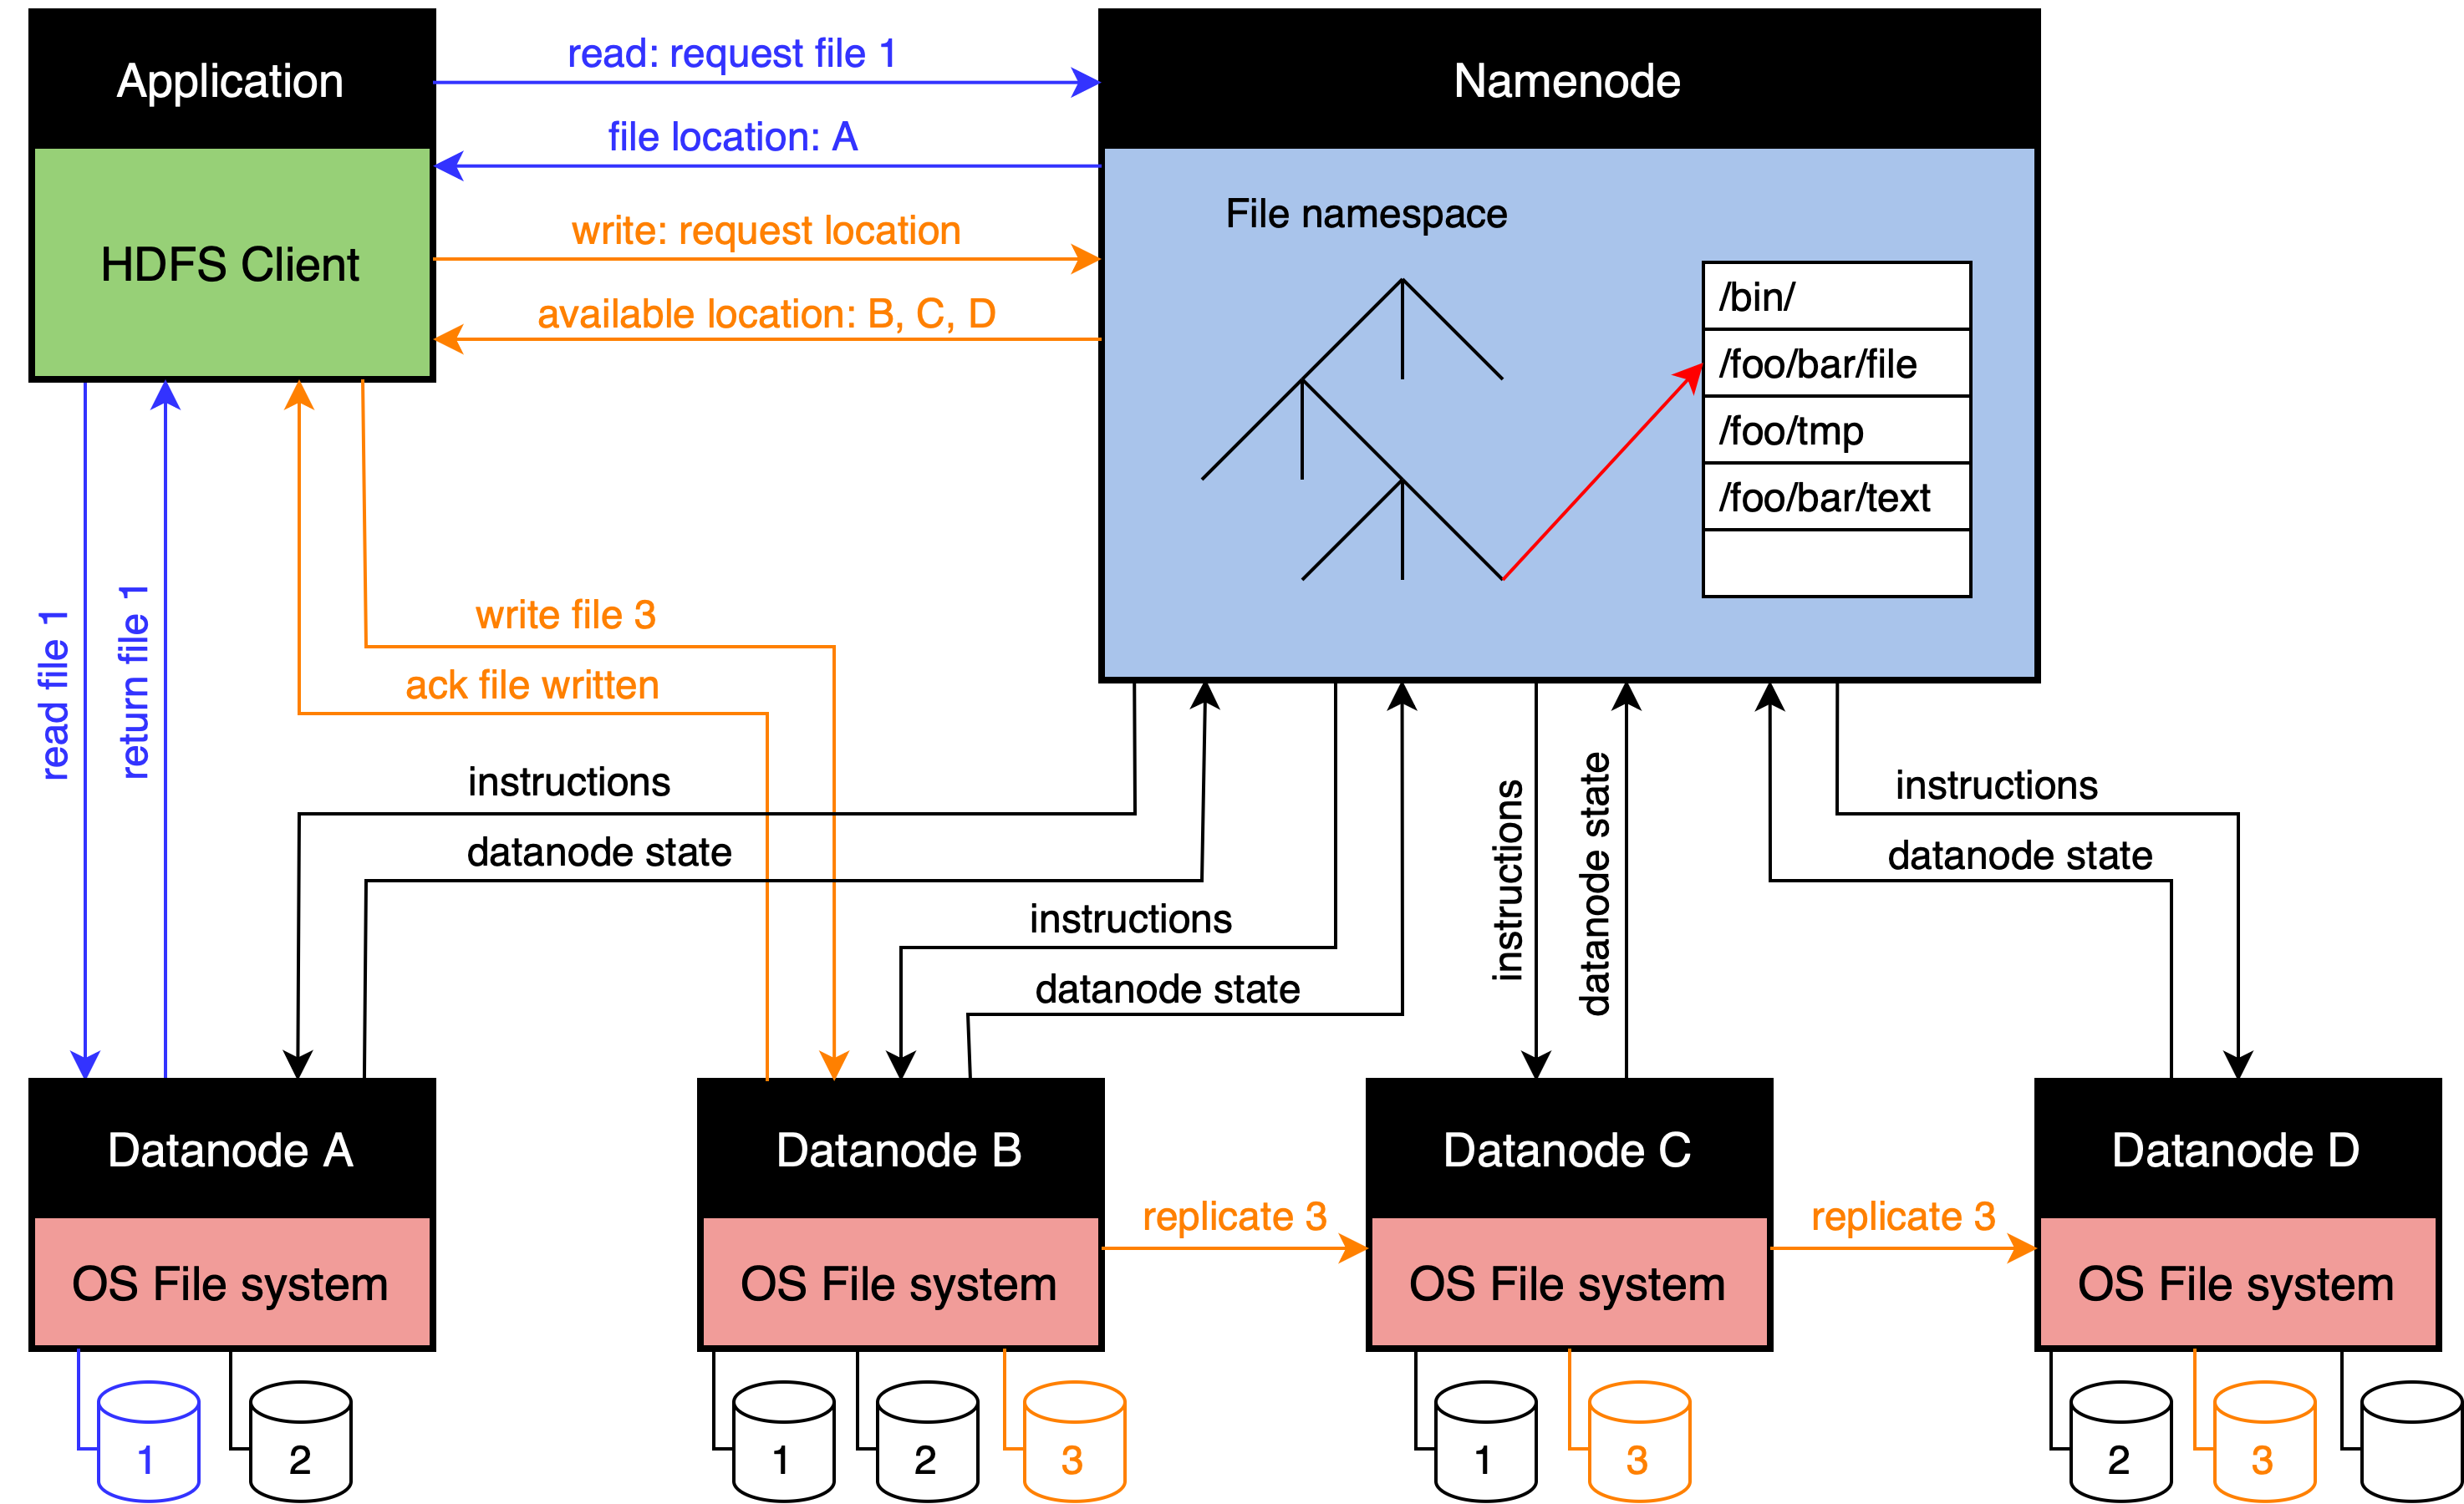
\includegraphics[width=\textwidth]{figures/2-background/HDFS.png}
    \end{center}
    \caption[Hadoop Distributed File System architecture]{\glsentryfull{HDFS} architecture displaying in different colors basic operations: read (blue), write (orange) and Namenode-Datanodes management messages (black). Note: for representation simplicity files are not segmented into blocks. Diagram inspired by the Data-intensive Computing lectures at KTH by Prof. A. H. Payberah. Course website available at \url{https://www.kth.se/student/kurser/kurs/ID2221?l=en}.}
    \label{fig:hdfs}
\end{figure}
 
\subsection{\glsfmtshort{HopsFS} as an \glsfmtshort{HDFS} evolution}

\gls{HopsFS} is \gls{HDFS} improved release first presented at the 15th USENIX conference in 2017 \cite{niaziHopsFSScalingHierarchical2017}. \gls{HopsFS} stores the metadata in an external NewSQL database with high throughput and low operation latency called RonDB~\footnote{Project's website available at \url{https://www.rondb.com}}. This enables this storage solution to avoid having all metadata in a single Namenode, but allowing for Namenode replication, having the same metadata on RonDB. This solution proved to have from sixteen up to thirty-seven times the performance on \gls{HDFS} thanks to its ability to scale according to metadata being stored, and also on similar setups where the same resources are being utilized. 

\gls{HopsFS} is one of the core technologies on which the Hopsworks Feature Store is built. While the system has not seen more widespread use, it is extremely impactful in its current applications, contributing to making Hopsworks "outperform existing cloud feature stores for training and online inference query workloads" \cite{10.1145/3626246.3653389}. 

\subsection{\glsfmtshort{HDFS} alternatives: Cloud object stores}

Thanks to its high scalability and low cost (Section \ref{subsec:file_vs_obj_vs_block}) object storage has been widely adopted to store large quantities of unstructured data. Starting with \gls{AWS} in 2006 with its S3 service, a lot of other vendors started offering cloud object storage services. The main advantages of using cloud resources are related to their elasticity that combined with object storage capability enable users to use as much storage as they need and be billed for what was used. 

\gls{HDFS} was first released in 2006, and so it evolved in parallel with cloud objects storage solutions. While \gls{HDFS} was widely adopted for on-premise solutions, more and more businesses migrated their operations to cloud services. Nowadays, cloud object storage like \gls{AWS}'s S3, Google's \gls{GCS} and Microsoft's Azure are widely used and libraries, e.g. delta-rs, prioritize support for these platforms as they are widely adopted. \gls{HDFS} and its evolutions, e.g. \gls{HopsFS}, still see use, but it fits more specific use cases, as the convenience of a cloud service is highly valued by the market.